%%% -*- Coding: utf-8-unix; Mode: latex; TeX-master: "paper"; ispell-local-dictionary: "american" -*-

\documentclass[preprint,12pt]{elsarticle}

%% Use the option review to obtain double line spacing
%% \documentclass[preprint,review,12pt]{elsarticle}

%% Use the options 1p,twocolumn; 3p; 3p,twocolumn; 5p; or 5p,twocolumn
%% for a journal layout:
%% \documentclass[final,1p,times]{elsarticle}
%% \documentclass[final,1p,times,twocolumn]{elsarticle}
%% \documentclass[final,3p,times]{elsarticle}
%% \documentclass[final,3p,times,twocolumn]{elsarticle}
%% \documentclass[final,5p,times]{elsarticle}
%% \documentclass[final,5p,times,twocolumn]{elsarticle}

%% if you use PostScript figures in your article
%% use the graphics package for simple commands
%% \usepackage{graphics}
%% or use the graphicx package for more complicated commands
%% \usepackage{graphicx}
%% or use the epsfig package if you prefer to use the old commands
%% \usepackage{epsfig}

\usepackage{graphicx}
\usepackage{amsmath}
\usepackage{mathptmx}
%\usepackage{bbb}
\usepackage{amssymb}
\usepackage[utf8]{inputenc}
\usepackage[T1]{fontenc}
\usepackage{txfonts}
\usepackage{subfigure}
%\usepackage {color}
%\usepackage{multirow}
%\usepackage{topcapt}
%\usepackage{bbm}
\usepackage[ruled,linesnumbered,lined]{algorithm2e}
%\usepackage{subfig}
\usepackage{morefloats}


%% The amssymb package provides various useful mathematical symbols
%%\usepackage{amssymb}
%% The amsthm package provides extended theorem environments
%% \usepackage{amsthm}

%% The lineno packages adds line numbers. Start line numbering with
%% \begin{linenumbers}, end it with \end{linenumbers}. Or switch it on
%% for the whole article with \linenumbers after \end{frontmatter}.
%% \usepackage{lineno}

%% natbib.sty is loaded by default. However, natbib options can be
%% provided with \biboptions{...} command. Following options are
%% valid:

%%   round  -  round parentheses are used (default)
%%   square -  square brackets are used   [option]
%%   curly  -  curly braces are used      {option}
%%   angle  -  angle brackets are used    <option>
%%   semicolon  -  multiple citations separated by semi-colon
%%   colon  - same as semicolon, an earlier confusion
%%   comma  -  separated by comma
%%   numbers-  selects numerical citations
%%   super  -  numerical citations as superscripts
%%   sort   -  sorts multiple citations according to order in ref. list
%%   sort&compress   -  like sort, but also compresses numerical citations
%%   compress - compresses without sorting
%%
%% \biboptions{comma,round}

% \biboptions{}

\journal{European Journal of Operational Research}

\begin{document}

\begin{frontmatter}

%% Title, authors and addresses

%% use the tnoteref command within \title for footnotes;
%% use the tnotetext command for the associated footnote;
%% use the fnref command within \author or \address for footnotes;
%% use the fntext command for the associated footnote;
%% use the corref command within \author for corresponding author footnotes;
%% use the cortext command for the associated footnote;
%% use the ead command for the email address,
%% and the form \ead[url] for the home page:
%%
%% \title{Title\tnoteref{label1}}
%% \tnotetext[label1]{}
%% \author{Name\corref{cor1}\fnref{label2}}
%% \ead{email address}
%% \ead[url]{home page}
%% \fntext[label2]{}
%% \cortext[cor1]{}
%% \address{Address\fnref{label3}}
%% \fntext[label3]{}

\title{Evolutionary Algorithms for Multi-Objective Portfolio Optimization}

%% use optional labels to link authors explicitly to addresses:
%% \author[label1,label2]{<author name>}
%% \address[label1]{<address>}
%% \address[label2]{<address>}

\author[agh]{Rafa{\l} Dre{\.z}ewski}
\author[agh]{Krzysztof Doroz}

\address[agh]{AGH University of Science and Technology, Department of
  Computer Science Krakow, Poland}

\begin{abstract}

Algorithms based on process of natural evolution are widely used to solve multi-objective optimization problems.
This study shows how genetic algorithms, co-evolutionary algorithms and co-evolutionary multi-agent systems deal with portfolio optimization problem.
All mentioned algorithms are implemented and compared with each other and trend following approach.
Historical data is used to assess their performance.

\end{abstract}

\begin{keyword}
%% keywords here, in the form: keyword \sep keyword

multi-objective optimisation \sep portfolio optimisation \sep genetic algorithms \sep co-evolutionary algorithms 
\sep co-evolutionary multiagent systems

%% MSC codes here, in the form: \MSC code \sep code
%% or \MSC[2008] code \sep code (2000 is the default)

\end{keyword}

\end{frontmatter}

%%
%% Start line numbering here if you want
%%
% \linenumbers

%----------------------------------------------------------------------------%
%%% -*- Coding: utf-8-unix; Mode: latex; TeX-master: "paper"; ispell-local-dictionary: "american" -*-

\section{Introduction}
\label{sec:introduction}

    The portfolio optimization problem is of great importance to each investor willing to risk
their money in order to get potential benefits exceeding interest rates.
Before 1950s, people relied on common sense, experience or even premonition to construct their portfolios.
Then the scientists \cite{MPT} were able to formulate theories establishing the relation between risk and potential
return of the investment.
Finally, investors had solid tools at hand to ease the uneasy process of investing money.
Obviously proposed theories will not make each of us a millionaire.
They can merely be used as a yet another source of analytical information that can be taken into consideration.

\subsection{Multi-objective optimization}

\label{sec:multi}

The main goal of optimization is to find the very best solution from a most likely infinite set of possibilities.
Optimization procedure relies on finding and comparing feasible solutions until no better solution can be found.
Each solution can be classified as good or bad in terms of a specific objective we are interested in.
E.g. we could define objective as the cost of fabrication, efficiency of a technological process, etc.
Contrary to single-objective optimization there is no clearly defined optimum, instead of that we have to deal with a set of trade-off optimal solutions.
They are generally known as Pareto-optimal solutions \cite{zitz1999a}.

Vast majority of real-world problems involve more than one objective.
That's why it is so crucial to develop methods to efficiently solve them 
\cite{zitz1999a}, \cite{Deb:2001:MOU:559152}.

Multi-objective optimization problem (MOOP) deals with more than one objective function.
It turns out that objectives are most likely contradictory which makes the MOOP difficult to solve.
In fact it is the most common situation we will ever encounter. 
Following \cite{Deb:2001:MOU:559152} - formal definition of MOOP is being defined as follows:

\begin{equation} 
MOOP \equiv
 \begin{cases}
     Minimize/Maximize  & f_{m}(\bar{x}), \text{ } m = 1,2...,M \\
     Subject \text{ } to  &  g_{j}(\bar{x}) \geq 0, \text{ } j = 1,2..., J  \\ 
			  &  h_{k}(\bar{x}) = 0, k = 0,1...,K \\
			  &  x_{i}^{(L)} \leq x_{i} \leq x_{i}^{(U)}, i = 1,2...,N
      
\end{cases}  
\end{equation}

These constraints and bounds ($g_{j}(x) , h_{k}(x) $ are constraint functions and there are $M$ objective functions) constitute a \emph{decision space}  
\cite{Deb:2001:MOU:559152}.
Any solution that satisfies all the constraints and bounds is called a \emph{feasible solution} \cite{Deb:2001:MOU:559152}.

It turns out that the set of feasible solutions is partially ordered.
In order to compare two solutions we introduce \emph{Pareto dominance} relation \cite{zitz1999a}:

\begin{equation}
\bar{x}_{A}  \prec \bar{x}_{B} \equiv
      \begin{cases}
     \exists{i \in 1..M} : f_{i}(\bar{x}_{A}) < f_{i}(\bar{x}_{B}) \\
     \neg (\exists{j \in 1..M} : f_{j}(\bar{x}_{A}) > f_{j}(\bar{x}_{B}))  \\ 
			  
      
\end{cases} 
\end{equation}

Solution that is not dominated by any other solution is called \emph{non-dominated}. 
The set of \emph{non-dominated} solutions is what we are actually trying to find while dealing with MOOPs.

\begin{figure}[ht]
  \begin{center}
    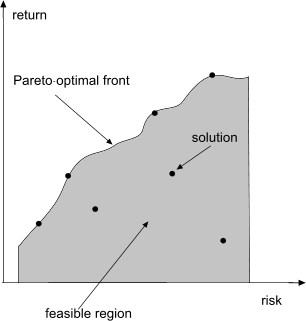
\includegraphics[scale=.9]{pareto_front.png}
  \end{center}
  \caption{Pareto-optimal front of portfolio optimization problem}
\end{figure}


Pareto-optimal front is the set of choices that are \emph{non-dominated} (\cite{drezewski2008coevolutionary}).
 


%%% -*- Coding: utf-8-unix; Mode: latex; TeX-master: "paper"; ispell-local-dictionary: "american" -*-

\section{Previous Research}
\label{sec:previous-research}

Many researchers worked on application of evolutionary algorithms to portfolio optimization problem.

Authors of \cite{Drezewski:2009:CMC:1533570.1533599} focused on comparison of evolutionary algorithms with multi-agent co-evolutionary algorithms.
They concluded that further research is needed as obtained results suggested that neither agent-based approach nor classical algorithms can obtain good results
for all kind of problems.

Evolutionary approach was compared with simple investing strategies and stock market index in \cite{Lipinski:2009:BRP:1574739.1574764}.
In some cases the proposed technique outperformed basic Buy\&Hold strategy as well as market index.

Co-evolutionary multi-agent system is presented in \cite{Drezewski:2009:MOT:1574739.1574761}.
The system was run against well-known test problems as well as portfolio optimization problem.
Results obtained from both tests proved the CoEMAS approach to be robust. 
%%% -*- Coding: utf-8-unix; Mode: latex; TeX-master: "paper"; ispell-local-dictionary: "american" -*-

\section{Evolutionary and Co-Evolutionary Algorithms for Portfolio
  Optimization}
\label{sec:system}

All algorithms mentioned in this chapter are implemented to actually calculate the best possible portfolio throughout a specified time period which
forces them to adjust to changing market's conditions and provide the trading strategy as we can follow portfolio's composition adjustments made on a daily 
basis.  


\subsection{Genetic Algorithm}
\label{GA}

Genetic algorithms (GAs) are well-known and popular method of dealing with MOOPs.
They are described in great details in \cite{Mitchell01}.

Every time we try to use GAs to solve a problem we have to adjust it accordingly.
In our implementation each potential solution should be encoded inside a chromosome. 
Each chromosome represents portfolio composition (it is a normalized vector of double values representing percentage share of each stock).
Before first round of computation, the entire population is created from scratch using random values in chromosomes.

The following modified GA operations have been implemented:
\begin{description}
  \item [mutation]
      - mutation operator changes exactly one value $ \alpha_{i} $ representing percentage share of a specific stock $i$ (each time the value $i$ is chosen randomly)
      to $\alpha_{i}'$ ($\alpha_{i}' \in (0,1)$ is chosen randomly). 
      After that, we have to normalize the vector.
      \emph{Mutation\_coefficient} (\emph{mutation\_coefficient} $ \in (0,1)$ ) determines what part of the population will be subjected to mutation operator.
  \item [selection]
      - \emph{breeding\_coefficient} ( \emph{breeding\_coefficient} $ \in (0,1)$ ) determines what part of population will be subjected to crossover operator, selection is based on 
      fitness function (only the fittest part of the population will be selected);
  \item [crossover]
      - after selection chromosomes eligible for reproduction, each pair of chromosomes are subjected to crossover operator. As a result new chromosomes are created (each pair
      produces two new chromosomes) and added to population. Crossover choose points $left$  and $right$ (both are chosen randomly) which cut parent's chromosomes in the way
      presented in figure~\ref{fig:parents}. Children are created according to a process shown in figure~\ref{fig:children}.
      
       \begin{figure}[H]
	    \begin{center}
	      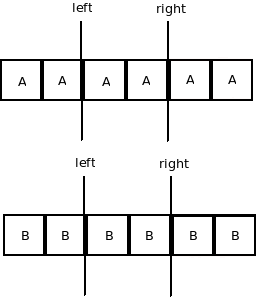
\includegraphics[scale=.3]{parents.png}
	    \end{center}
	    \caption{Example of parent's chromosomes split into 3 parts}
	    \label{fig:parents}
	  \end{figure}

	  \begin{figure}[H]
	    \begin{center}
	      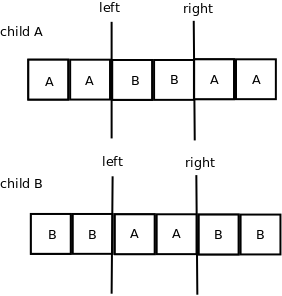
\includegraphics[scale=.3]{children.png}
	    \end{center}
	    \caption{Children's chromosomes contain mixed parent's genetic material}
	    \label{fig:children}
	  \end{figure}

\end{description}

Apart from that, extinction mechanism has been implemented.
At the end of each GA round a part of the population that has the lowest fitness is exterminated.
\emph{Extinction\_coefficient} determines what part of population will be subjected to extinction.
 
\subsubsection{Pseudocode}

Pseudocode of GA is presented in Algorithm~\ref{genetic_pseudo}.
We start by evaluating each chromosome using fitness function described in \ref{sec:gen_fitness_fun}, which uses current stock prices.
The fittest individuals are allowed to reproduce (this is further controlled by \emph{breeding\_coefficient}).
New individuals are merged to existing population.
After that, mutation is applied to a part of the least fit population to assure that population is diverse (in fact it is a way of implementing $reinitialization$
method, mentioned in \cite{zitz1999a}) and we do not miss any potentially better solutions.
Then we destroy some of the worst fit individuals which is useful because we can control the overall population size and we get rid of individual with chromosomes
not likely being successful in the future.
Finally, we return the best individual which becomes our trading strategy for next day (we adjust our current portfolio to the fittest individual solution). 


\begin{algorithm}
  \SetKwData{returnOrientedSubpopulation}{returnOrientedSubpopulation}
  \SetKwData{riskOrientedSubpopulation}{riskOrientedSubpopulation}
  \SetKwData{parents}{parents}
  \SetKwData{offspring}{offspring}
  \SetKwData{population}{population}
  \SetKwData{mutants}{mutants}
  \SetKwFunction{evaluate}{evaluate}
  \SetKwFunction{initialise}{initialise}
  \SetKwFunction{selectParents}{selectParents}
  \SetKwFunction{crossover}{crossover}
  \SetKwFunction{merge}{merge}
  \SetKwFunction{mutateLeastFitIndividuals}{mutateLeastFitIndividuals}
  \SetKwFunction{extinctLeastFitIndividuals}{extinctLeastFitIndividuals}
  \SetKwInOut{Input}{input}\SetKwInOut{Output}{output}
 
  \BlankLine
  \initialise{\population} \;
  
  \ForEach{$day$}{ 

      \ForEach{$individual$ $\in$ \population}{
	  \evaluate($individual$)\;
      }
     
      \parents $\leftarrow$  \selectParents{\population} \;
      \offspring $\leftarrow$ \crossover{\parents} \;
      \population  $\leftarrow$ \merge{\offspring, \population} \;

      \mutateLeastFitIndividuals{\population} \;

      \ForEach{$individual$ $\in$ \population}{
	  \evaluate($individual$)\;
      }

      \extinctLeastFitIndividuals{\population} \;
      \Return{the fittest individual} 
  }
  \caption{GA pseudocode}\label{genetic_pseudo}
\end{algorithm}




\subsubsection{Fitness function}
\label{sec:gen_fitness_fun}

Fitness is calculated according to the following formula (for portfolio with $N$ stocks):

\begin{equation}
    \gamma_{day} =  \sum_{i=1}^{N} {  \alpha_{i} * \frac{price(i,day)}{price(i,day - 1)} }
\end{equation}

where:

\begin{description}
  \item [$\gamma_{day}$] 
      is the value of the portfolio's fitness calculated for specific $day$;
  \item [$\alpha_{i}$]
      is the percentage share of a specific stock $i$ in the whole portfolio;
  \item [$price(i,day)$]
      returns the price of stock $i$ for a specific $day$.
\end{description}

Clearly, the fitness function favours the portfolios which have the highest day-to-day increase in value.
Of course such method of calculating fitness has many drawbacks e.g. it completely omits the aspect of risk associated with investing in highly volatile stocks.
However, it turns out that in spite of this obvious flaw the algorithm is performing quite well.  

\subsection{Co-evolutionary system}
\label{sec:co-evol-sys}

Contrary to \ref{GA}, in this approach two subpopulations coexist side by side.
Each individual represents potential solution to portfolio optimization problem.
Risk oriented subpopulation tries to optimize on risk (the lower risk value the better), whereas the return oriented subpopulation tries to maximize expected return.
Usually the greater the expected return the riskier the investment so our solutions will involve some trade-offs.
However that should not startle us, as we have already predicted in \ref{sec:multi} that optimization under such circumstances is not easy.

As presented in figure~\ref{fig:co-evol}, reproduction is allowed only between members of different subpopulations.
Not every member of a particular subpopulation is allowed to reproduce - only the fittest (fitness of a particular member depends on the subpopulation it belongs to - the fittest one
 in one subpopulation would probably be considered as one of the weakest in the other one).
Thanks to this approach the offspring that is created is very diverse.
In fact it is an application of $restricted$ $mating$ \cite{zitz1999a}.
Some part of the weakest members of both subpopulations is subjected to extinction.
Because of that we do not end up with too big population full of useless solutions.
In place of extinct members, offspring of the fittest is introduced to both subpopulations.

Apart from that, some members are subjected to mutations in order to even further maintain subpopulation diversity.
The migration mechanism has the same purpose - to avoid local extrema.
It is also described as an $isolation$ $by$ $distance$ \cite{zitz1999a}.
Risk as well as expected return are calculated according to Capital Asset Pricing Model (described in \cite{CAPM}) .
 

\begin{figure}[ht]  
	    \begin{center}
	      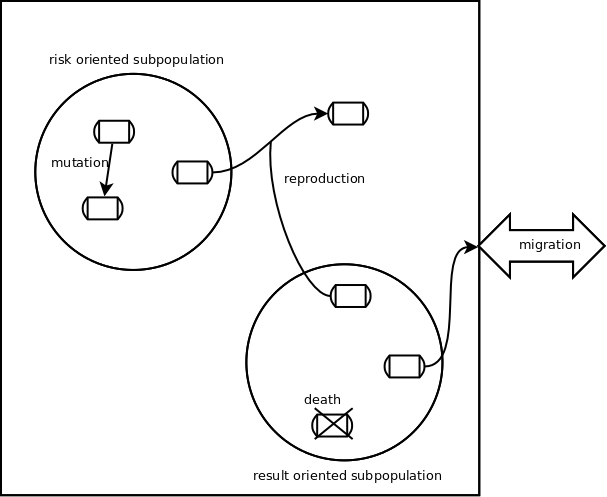
\includegraphics[scale=.2]{co-evol-2-sub.png}
	    \end{center}
	    \caption{Co-evolutionary system overview} 
	    \label{fig:co-evol}
	  \end{figure}

\subsubsection{Maintaining population diversity}

To sum up several mechanisms have been implemented to keep both subpopulations diverse:

\begin{itemize}
  \item crossover is allowed only between the fittest chromosomes from different subpopulations; 
  \item mutations introducing random genetic change;
  \item migration allows chromosomes to travel to different nodes.  
\end{itemize}

\subsubsection{Pseudocode}


\begin{algorithm}
  \SetKwData{returnOrientedSubpopulation}{returnOrientedSubpopulation}
  \SetKwData{riskOrientedSubpopulation}{riskOrientedSubpopulation}
  \SetKwData{parents}{parents}
  \SetKwData{offspring}{offspring}
  \SetKwData{population}{population}
  \SetKwData{mutants}{mutants}
  \SetKwFunction{evaluate}{evaluate}
  \SetKwFunction{initialise}{initialise}
  \SetKwFunction{selectParents}{selectParents}
  \SetKwFunction{recombine}{recombine}
  \SetKwFunction{merge}{merge}
  \SetKwFunction{mutateLeastFitIndividuals}{mutateLeastFitIndividuals}
  \SetKwFunction{extinctLeastFitIndividuals}{extinctLeastFitIndividuals}
  \SetKwInOut{Input}{input}\SetKwInOut{Output}{output}
 
  \BlankLine
  \initialise{\riskOrientedSubpopulation} \;
  \initialise{\returnOrientedSubpopulation} \;
  
  \ForEach{$day$}{ 

      \ForEach{$individual$ $\in$ \population}{
	  \evaluate($individual$)\;
      }
     
      \parents $\leftarrow$  \selectParents{\riskOrientedSubpopulation, \returnOrientedSubpopulation} \;
      \offspring $\leftarrow$ \recombine{\parents} \;
      \population  $\leftarrow$ \merge{\offspring, \riskOrientedSubpopulation, \returnOrientedSubpopulation} \;

      \mutateLeastFitIndividuals{\population} \;

      \ForEach{$individual$ $\in$ \population}{
	  \evaluate($individual$)\;
      }

      \extinctLeastFitIndividuals{\population} \;
      \Return{non-dominated solution} 
  }
  \caption{CEA pseudocode}\label{cea_pseudo}
\end{algorithm}

Contrary to GA, we are dealing with two populations (with different objectives) at once (see Algorithm~\ref{cea_pseudo}).
Apart from that, the pseudocode looks very similar.
Reproduction is only allowed between individuals from different subpopulations (which is a direct application of $restricted$ $mating$ method
 described in \cite{zitz1999a}).
To even further assure that populations remain diverse, we mutate part of the least fit individuals.
Extinction helps to control population size and get rid of useless individuals.
Non-dominated solution (in Pareto sense) is returned as a result.



\subsection{Co-Evolutionary Multi-agent System - CoEMAS}

Co-evolutionary Multi-agent System (CoEMAS) is the most sophisticated system that has been implemented.
As described in \cite{drezewski2008coevolutionary} and \cite{drezewski2008agent-based-cooperative} such systems need environment as well as a set of autonomous agents interacting with each other.
Potential solution to portfolio optimization problem is stored inside each agent.


\begin{figure}[ht]   
	    \begin{center}
	      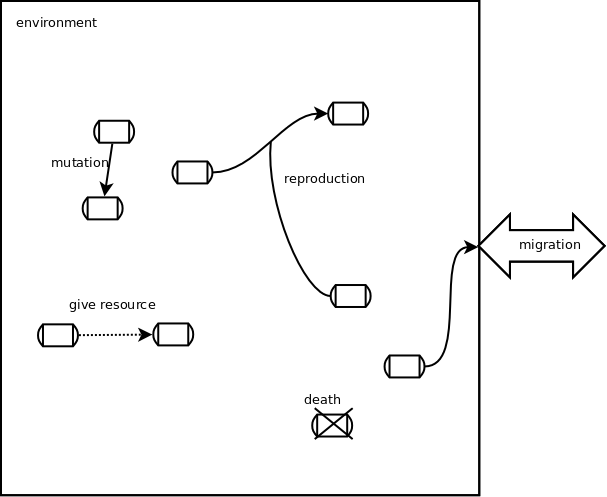
\includegraphics[scale=.2]{agent.png}
	    \end{center}
	    \caption{Overview of CoEMAS} 
	  \end{figure}

Contrary to \ref{sec:co-evol-sys} there are no subpopulations.
Instead of them we introduced individuals of two different species.
Each species focuses on different task:

\begin{itemize}
  \item species number 1 - tries to achieve the lowest risk possible;
  \item species number 2 - tries to achieve the highest expected return possible.
\end{itemize}

Risk as well as expected return is calculated due to Capital Asset Pricing Model (defined in \cite{CAPM}).

\subsubsection{Implemented actions}

Implemented actions that each agent can perform include:

\begin{description}
  \item [death]
      - if amount of resource that agent posseses is lower than threshold value the agent dies;
  \item [migration]
      - agent is allowed to migrate but the probability of this action is low;
  \item [reproduction]
      - agents from different species are allowed to reproduce provided that they both exceed the minimum amount of resource allowing to reproduce;
  \item [give/get]
      - agent can get resource from other, dominated agent;
  \item [recombination]
      - agents produce offspring by the means of recombination;
  \item [mutation]
      - mutation introduces random change to potential solution, normalization of solution vector is then required;
  \item [seek]
      - agents appropriate  to reproduction as well as get operation can be found thanks to this action.
\end{description}

Interactions between agents are implemented in the following way:
\begin{itemize}
  \item co-evolution is implemented as a sequence of \emph{turns};
  \item in each \emph{turn} every agent perform its action (action to perform at any particular turn is chosen with some well defined probability, e.g. there is a 10\% chance that agent will try to find
	a partner to reproduce, 60\% chance that the agent will try to get some resource from dominated agent);
  \item when every agent performed some action the \emph{turn} ends and entire population of agents is checked whether some of them should die (not enough resource left after other agents got resource
	from it).
\end{itemize}


Each agent performs one of the above actions with some probability.

\subsubsection{Pseudocode}


% \STATE randomly INITIALISE agents of two different species (risk oriented and return oriented) 
% \FORALL{ $day$ }
% 
%   \FOR{$round = 1$ $to$  $number\_of\_rounds$}  
%       \FORALL{ $agent$ $\in$ population }
%   \STATE choose a profile for $agent$
%   \STATE $agent$ should act according to a selected profile  
%       \ENDFOR
%   \ENDFOR
%   \RETURN non-dominated agent as a solution  
% \ENDFOR


\begin{algorithm}
  \SetKwData{Profile}{profile}\SetKwData{This}{this}\SetKwData{Up}{up}
  \SetKwFunction{Union}{Union}\SetKwFunction{chooseProfile}{chooseProfile}
  \SetKwInOut{Input}{input}\SetKwInOut{Output}{output}
 
  \BlankLine
  \emph{randomly INITIALISE agents of two different species (risk oriented and return oriented)}\;
  \ForEach{$day$}{ 

    \For{$round\leftarrow 1$ \KwTo $number\_of\_rounds$}{\label{forins}
      \ForEach{$agent$ $\in$ population}{
      
      \Profile$\leftarrow$ \chooseProfile{}\;

      \If(){\Profile is $resource\_profile$ }{\label{lt}
        perform actions specified in $resource\_profile$ 
      }

      \If(){\Profile is $reproduction\_profile$ }{\label{lt}
        perform actions specified in $reproduction\_profile$ 
      }

      \If(){\Profile is $migration\_profile$ }{\label{lt}
        perform actions specified in $migration\_profile$ 
      }
      
    }
}
  }
  \caption{CoEMAS pseudocode}\label{coemas_pseudo}
\end{algorithm}

Pseudocode of CoEMAS is presented in Algorithm~\ref{coemas_pseudo}.

Profiles are chosen with following probabilities:
\begin{itemize}
  \item $resource$ $profile$ - with probability 0.6;
  \item $reproduction$ $profile$ - with probability 0.2;
  \item $migration$ $profile$ with probability 0.1;
  \item $mutation$ $profile$ with probability 0.1.
\end{itemize}

Similarly to \ref{sec:co-evol-sys}, mutation is used as a mean of maintaining population diversity.

%%% -*- Coding: utf-8-unix; Mode: latex; TeX-master: "paper"; ispell-local-dictionary: "american" -*-

\section{Trend following}
\label{sec:trend-following}

The concept of price as the trading cue lays the foundations for trend following (TF). 
Contrary to other trading strategies based on fundamental analysis (which use factors like: overall state of the economy, interest rates, production, etc. to predict stock price)
TF use only price as the key trading variable. 

Trend following basically does not try to predict when the trend will occur. 
Instead of that, trend followers will react to the market's movement and adapt accordingly.
This strategy simply analyses stock prices and decides whether the current situation is suitable for buying or selling a specific stock.
Market breakouts are a great buying opportunities, on the other hand when you recognize that you are wrong you exit immediately in order to cut losses.
Set of predefined rules decides  whether to take any action (they should recognize when the trend starts as well as when to exit) so the entire process can be easily automated.
Such rules are quite simple but disciplined execution of them could lead to achieving spectacular returns year after year.
It is all about cutting the losses and letting the profits run.
Many leading hedge funds successfully use strategies based on trend following to manage their portfolios \cite{Trend01}.  

\begin{figure}[ht]
  \begin{center}
    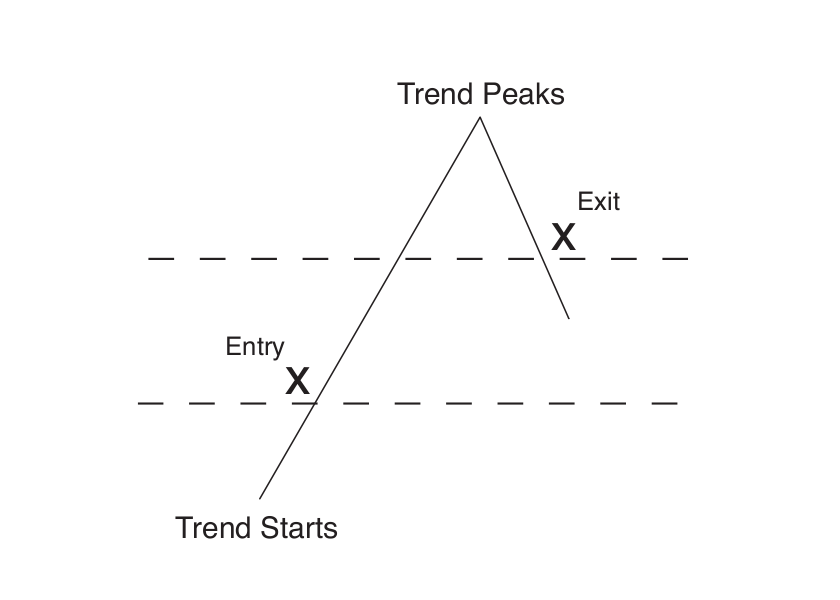
\includegraphics[scale=.2]{trend_following.png}
  \end{center}
  \caption{Simple example of how trend following works in practise (\cite{Trend01})}
\end{figure}

Another advantage of this investing method is the fact that investor does not have to know much about what is being traded (it could be stocks, oil, gold, etc.).
Normally, people tend to gather some information about the company they are willing to invest in. 
They analyse its market situation, competitors, financial performance, etc. which is time consuming, especially for someone who is not a professional trader.
With trend following we just have to focus on elaborating trading rules that should reflect our trading strategy.
After that, we can automate the decision making process by designing and implementing our own trading system.   

\subsection{Types of trends}
\label{sec:types_of_trends}

There are three main types of trends:

\begin{enumerate}
  \item \textbf{Short-term trend}: any price movement that occurs over a few hours or days.
  \item \textbf{Intermediate-term trend}: general movement in price data that lasts from three weeks to six months.
  \item \textbf{Long-term trend}: any price movement that occurs over a significant period of time, often over one year or several years.
\end{enumerate}



\subsection{Designing trading system based on trend following} 

Following \cite{Trend01}, the core of each trading system based on trend following strategy is a set of rules governing each buy/sell decision.
More specifically we have to devise rules to answer the following questions:

\begin{itemize}
  \item how much money are we willing to put on a single trade;
  \item when to exit (what kind of losses are acceptable);
  \item when to enter (when the trend has started); 
  \item what markets are we interested in and how to split money between them (we would like to have a diverse portfolio (stocks, gold, etc.)).
\end{itemize}

These rules should reflect our investing style.

Simple Moving Average (SMA) is especially useful to highlight longer-term trends in a set of data points \cite{Trend01}.

SMA is formulated as the unweighted mean of the previous $N$ data points \cite{Trend01}:

\begin{equation}
    SMA_{today,N} = \frac{\sum_{i=1}^{N}p_{today - i}}{N}
\end{equation}

\begin{description}
  \item [$p_{j}$] 
    value of data on day $j$
\end{description}

In this case, data points will represent closing stock prices. 
 


\textbf{Entry points:}
  \begin{itemize}
    \item Simple moving average (SMA) of last $N$ days is greater than SMA of last $M$ days ($N$ < $M$);
    \item Current stock price is max of last $N$ days (that is usually a good indicator of lucrative opportunity on the market).
  \end{itemize}

As soon as at least one of the above conditions is satisfied we go long (we buy a particular asset).


\textbf{Exit points:}
  \begin{itemize}
    \item Losses on a single trade are greater than 2 \% (this rule is used to quickly abandon an investment that we were wrong about its trend direction,
	  the amount of tolerable loss solely depends on our strategy and does not have to be exactly 2\%);
    \item Simple moving average (SMA) of last $N$ days is lesser than SMA of last $M$ days ($N$ < $M$).
  \end{itemize}

As soon as the exit condition is satisfied we go short (we sell a particular asset).
 
Obviously the above rules are very simple and quite straightforward.
Nonetheless, the system based on them proves to be robust, as shown in chapter \ref{sec:experiments}.
   
By manipulating the value of $N$ we can seek out different types of trends, as mentioned in \ref{sec:types_of_trends}. 

\subsection{Pseudocode}

Algorithm~\ref{fig:tf_pseudo} shows pseudocode of trend following. It uses the following functions:


\begin{description}

\item[SMA(i,N)]
  calculates Simple Moving Average for stock $i$, $N$ last days are taken into account  
\item[go\_short(i)]
  sell stock $i$
\item[go\_long(i)]
  buy stock $i$
\item[get\_current\_stock\_price(i, day)]
  returns stock $i$ price for specific $day$ 
\item[get\_most\_recent\_trade\_price(i)]
  returns the price we paid for stock $i$ (we have stock $i$ in our portfolio)
\item[max(i,N)]
  returns the maximum price for stock $i$ in the last $N$ days
\item[N, M, maximal\_value\_loss]
  modifiable parameters
\end{description}
% 


% \begin{algorithmic}
% 
% \STATE $maximal\_value\_loss \gets 0.98$
% 
% \FOR{$day = 1$ to $max\_day$} 
% 
%   \FOR{$i = 1$ to $number\_of\_stocks$}
% 
%     \IF {$ get\_most\_recent\_trade\_price(i) < maximal\_value\_loss * get\_current\_stock\_price(i, day) $} 
% 	    \STATE $go\_short(i)$
%     \ELSE
% 	    \IF {$SMA(i,N) < SMA(i,M)$}
% 		    \STATE $go\_short(i)$
% 	    \ENDIF
%     \ENDIF
% 
%     \IF {$SMA(i,N) > SMA(i,M)$} 
% 	    \STATE $go\_long(i)$
%     \ELSE
% 	    \IF {$max(i,N)) <= get\_current\_stock\_price(i, day)$}
% 		    \STATE $go\_long(i)$
% 	    \ENDIF
%     \ENDIF
% 
%   \ENDFOR
% 
% \ENDFOR
% 
% \end{algorithmic}

\begin{algorithm}
  \SetKwData{parents}{parents}
  \SetKwData{maxDays}{maxDays}
  \SetKwData{numberOfStocks}{numberOfStocks}
  \SetKwData{maximumValueLoss}{maximumValueLoss}
 
  \SetKwFunction{SMA}{SMA}
  \SetKwFunction{getMaxStockPrice}{getMaxStockPrice}
  \SetKwFunction{goShort}{goShort}
  \SetKwFunction{goLong}{goLong}
  \SetKwFunction{getMostRecentTradePrice}{getMostRecentTradePrice}
  \SetKwFunction{getCurrentStockPrice}{getCurrentStockPrice}
  \SetKwFunction{mutateLeastFitIndividuals}{mutateLeastFitIndividuals}
  \SetKwFunction{extinctLeastFitIndividuals}{extinctLeastFitIndividuals}
  \SetKwInOut{Input}{input}\SetKwInOut{Output}{output}
 
  \Input{$N$, $M$}
  \BlankLine
  \maximumValueLoss $\leftarrow$ 0.98 \;
  
  \For{$day\leftarrow 1$ \KwTo \maxDays}{

     \For{$i\leftarrow 1$ \KwTo \numberOfStocks}{
      
      \BlankLine

	\If(){\getMostRecentTradePrice{$i$} < \maximumValueLoss * \getCurrentStockPrice{$i$, $day$} }{
	  \goShort{$i$} \;
      }
      \ElseIf{\SMA{$i$, $N$} < \SMA{$i$, $M$}}{
	   \goShort{$i$} \;
	}

      \BlankLine

      \If(){\SMA{$i$, $N$} > \SMA{$i$, $M$} }{
	  \goLong{$i$} \;
      }
      \ElseIf{\getMaxStockPrice{$i$, $N$} <= \getCurrentStockPrice{$i$, $day$} }{
	   \goLong{$i$} \;
	}


    }
  }
  \caption{Trend following pseudocode}\label{fig:tf_pseudo}
\end{algorithm}

%%% -*- Coding: utf-8-unix; Mode: latex; TeX-master: "paper"; ispell-local-dictionary: "american" -*-

\section{Experimental Results}
\label{sec:experiments}

\subsection{First Set of Tests}
\label{sec:first_set_of_tests}

First set of tests uses historical data from year 2010 (data of 3 different stocks have been used). 
Portfolio contained 3 assets (they are one of the biggest companies present on WSE):

\begin{itemize} 
  \item KGHM;
  \item TPSA;
  \item PKO BP.
\end{itemize}

Multi-agent platform has been used to run algorithms.
It was configured in the following way: 

\begin{itemize}
  \item configured to simulate trading strategy throughout the entire year 2010;
  \item all investing decisions are solely based on results from algorithms;
  \item migration mechanism between Computing Nodes has been enabled;
  \item two Computing Nodes (with appropriate algorithms) have been used to obtain results.
\end{itemize}

Trend following algorithm has been tested without multi-agent running platform as it is a standalone R script.
Apart from that, it is completely deterministic algorithm so each time we run it, we will get the same results.

\subsection{Trend Following}

\subsubsection{Short-term trend results}
\label{short-term}

As described in \ref{sec:trend-following}, we can adjust our trading rules to seek out short-term trends
 (by changing the values of $N$ and $M$ in the \emph{Simple Moving Average} method).
With values $N = 10$, $M = 20$ the SMA method focused on short-term trends.
 

  

\begin{figure}[htb]
  \subfigure[short-term trends]{
  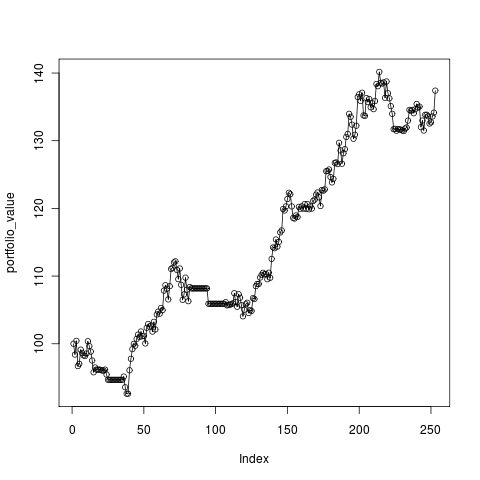
\includegraphics[scale=.33]{rplot0.png}
\label{fig:trend-short}}
  \subfigure[intermediate-term trends]{
  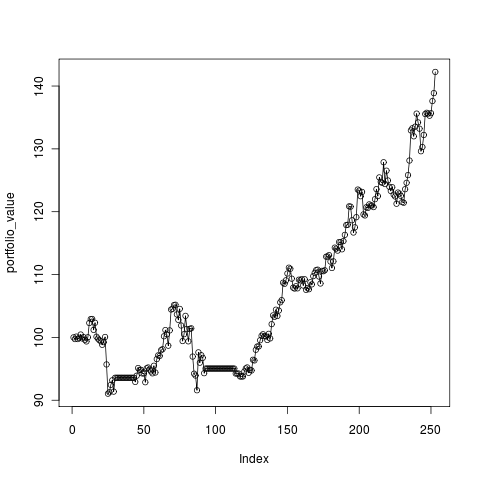
\includegraphics[scale=.33]{rplot.png}
  \label{fig:trend-int}
}
  \caption{Charts showing portfolio value in time for TF using short-term and intermediate-term trends}
\label{fig:TF}
\end{figure}

There are easily visible periods of time (figure~\ref{fig:trend-short}) when the portfolio value is not changing. 
It is a time when our portfolio does not contain any assets (but we still have money). 
After a while, conditions change and trend following algorithm decides to buy some assets.


\subsubsection{Intermediate-term trend results}
\label{trend-foll-inter}

In this particular test (with values: $N = 20$, $M = 40$), trend following algorithm has been adjusted to focus on intermediate-term trends.
 


Results are presented in figure~\ref{fig:trend-int}, as can be seen they are slightly better compared with short-term trends approach.  

\subsubsection{Conclusions}

It turned out that focusing on short-term or intermediate-term trends leads to almost the same results.
Intermediate-term trend approach offers slightly better return from the investment.
In both cases we encountered periods of time when portfolio contained no assets because situation on the market was not good enough to invest in any of the available stocks.


%---------------------------------------------------------------------------

\subsection{Genetic algorithm}

The best results that we were able to obtain are presented in figure~\ref{fig:gen-algo}.
Apart from that, the average values of 5 runs are shown in figure~\ref{fig:gen-algo-ave-2010}.
As can be easily spotted the algorithm perform reasonably well on the average.

The following configuration was used:
\begin{itemize}
  \item $reproduction\_$ $coeff$ was set to 0.2;
  \item population size is 512;
  \item $mutation$ $\_$ $coeff$ was set to 0.1;
  \item $extinction$ $\_$ $coeff$ was set to 0.3.
\end{itemize}

\begin{figure}[htb]
  \subfigure[Chart showing value of our best portfolio in time for GA]{
  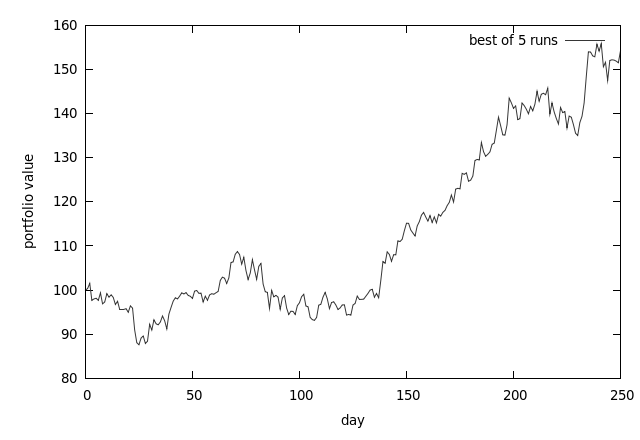
\includegraphics[scale=.3]{best_2010_gen.png}
\label{fig:gen-algo}}
  \subfigure[Chart showing average values of our portfolio in time for GA]{
  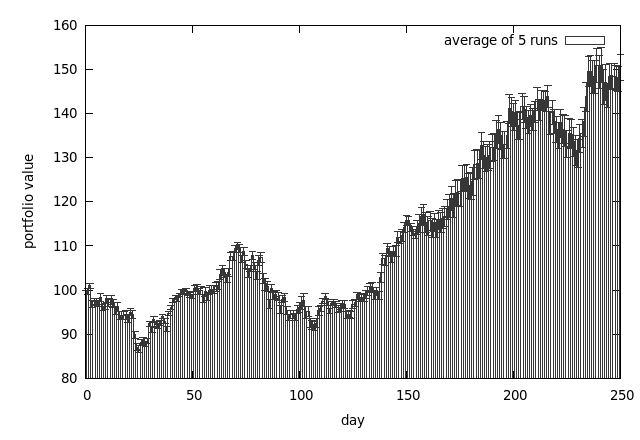
\includegraphics[scale=.3]{ave_2010_gen.png}
  \label{fig:gen-algo-ave-2010}
}
  \caption{Charts showing average and best portfolio values obtained for GA}
\label{fig:gen-algo-ave-2010-com}
\end{figure}





\subsection{Co-evolutionary algorithm}
\label{sec:co-evol-2}


Results presented in figure~\ref{fig:co_eval_return} clearly show that the return of our investment is much higher than any other algorithm could achieve.  
Analysing figure~\ref{fig:co_eval_risk} explains why the results are so good - the risk associated with our portfolio is substantially higher compared to other methods.
In this case algorithm was tuned to treat non-dominated solutions from return oriented subpopulation - this explains why the results provide so much return and risk. 

The following configuration was used:
\begin{itemize}
  \item $reproduction\_$ $coeff$ was set to 0.2;
  \item subpopulation size in each computing node was set to 64;
  \item number of computing nodes was set to 2;
  \item $mutation$ $\_$ $coeff$ was set to 0.1;
  \item $extinction$ $\_$ $coeff$ was set to 0.3.
\end{itemize}

\begin{figure}[htb]
  \subfigure[Chart showing value of our best portfolio in time for CEA]{
  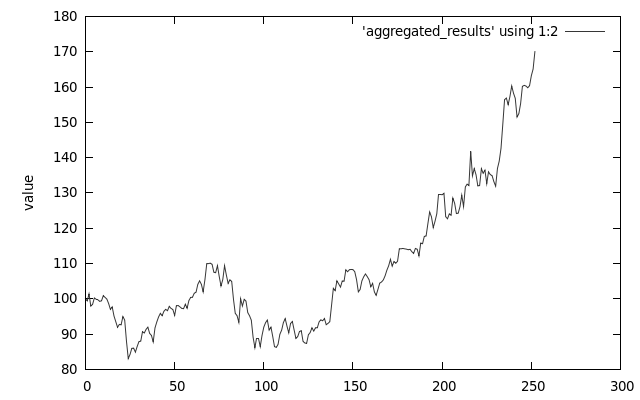
\includegraphics[scale=.3]{co-evol-value-oriented.png}
\label{fig:co_eval_return}}
  \subfigure[Chart showing average value of our portfolio value in time for CEA]{
  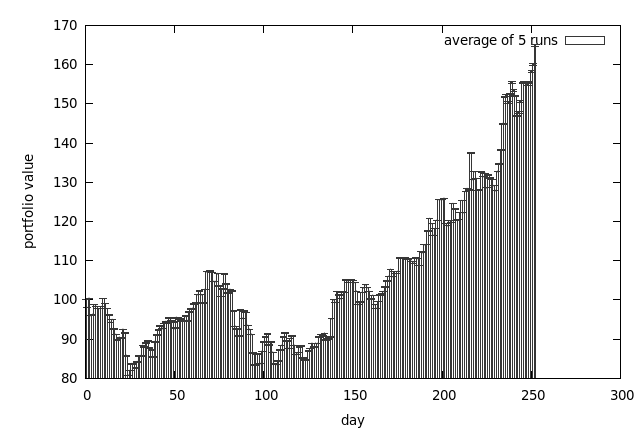
\includegraphics[scale=.3]{cea_ave_2010.png}
  \label{fig:co_eval_return}
}
  \caption{Charts showing average and best portfolio values obtained for CEA}
\label{fig:co-evol-ave-2010-com}
\end{figure}


\subsubsection{Pareto front}

Because co-evolutionary algorithm operates in terms of risk and return we can check if the non dominated solutions (in Pareto sense) are used to construct our portfolio.
Figure~\ref{fig:pareto_co_evol} shows the results of computation (results from a period of 6 days are presented for the sake of clarity). 
Portfolio is built according to the solutions that are connected with red line.
All of them are non dominated and all have the maximum return possible from all available feasible solutions at any particular day.

Solutions from two different computing nodes are shown.
It turns out that results from the second node are much better than from the first.
In fact all of the selected solutions come from the second one.

\begin{figure}[ht]
  \begin{center}
    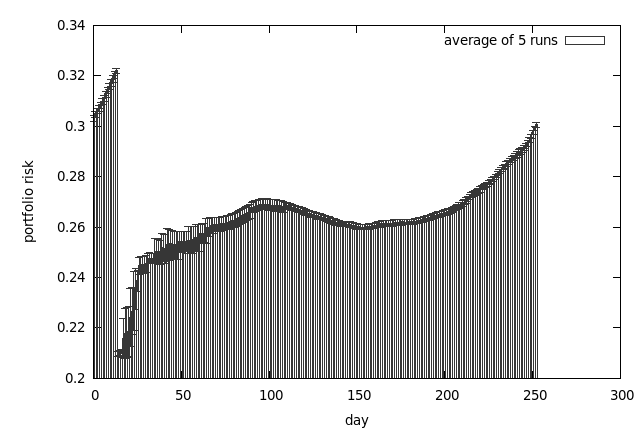
\includegraphics[scale=.3]{cea_ave_risk_2010.png}
  \end{center}
  \caption{Chart showing average value of risk in time for CEA}
  \label{fig:co_eval_risk}
\end{figure}

\begin{figure}[ht]
  \begin{center}
    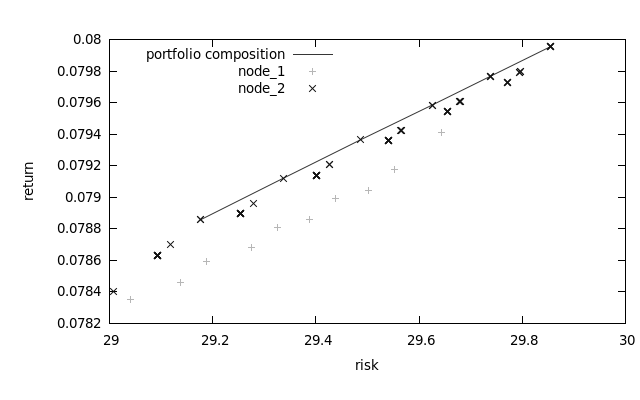
\includegraphics[scale=.3]{pareto_co_evol.png}
  \end{center}
  \caption{Chart showing the relation between return and risk of the particular solution}
  \label{fig:pareto_co_evol}
\end{figure}


\subsection{CoEMAS}

Figure~\ref{fig:agent_return} presents portfolio value in time while  figure~\ref{fig:agent_risk} presents the risk associated with our investments.
Returns are not so spectacular as in CEA but on the other hand the amount of risk we have to take is much lower.

The following configuration was used:
\begin{itemize}
  \item $reproduction\_$ $coeff$ was set to 0.2;
  \item each species was represented initially by 64 agents (in each computing node);
  \item number of computing nodes was set to 2;
  \item $mutation$ $\_$ $coeff$ was set to 0.1;
  \item $extinction$ $\_$ $coeff$ was set to 0.3.
\end{itemize}

\begin{figure}[htb]
  \subfigure[Chart showing value of our portfolio in time (CoEMAS)]{
  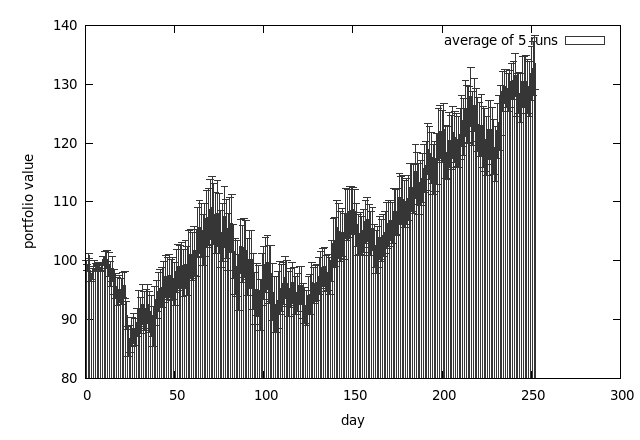
\includegraphics[scale=.33]{coemas_ave_2010.png}
\label{fig:agent_return}}
  \subfigure[Chart showing average value of risk in time (CoEMAS)]{
  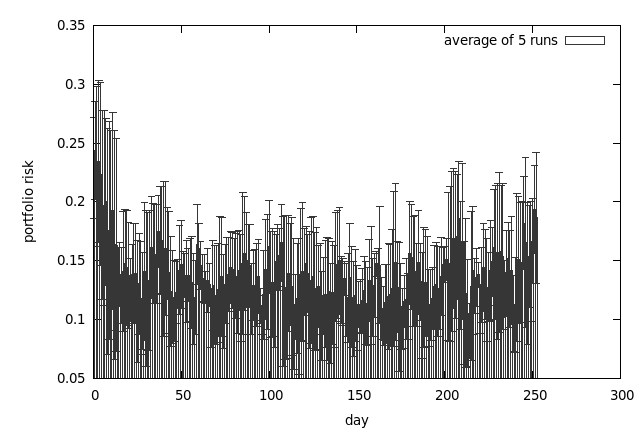
\includegraphics[scale=.33]{coemas_ave_risk_2010.png}
  \label{fig:agent_risk}
}
  \caption{Charts showing results for CoEMAS}
\label{fig:CoEMAS_1}
\end{figure}


\subsubsection{Pareto front}

CoEMAS like co-evolutionary algorithm gives us the opportunity to check if the non dominated solutions (in Pareto sense) are used to construct our portfolio.
Figure~\ref{fig:pareto_coemas} shows the results of computation (because of the fact that populations are quite numerous,
 results from a period of 3 days are presented for the sake of clarity). 
Solutions chosen to be a blueprint for our portfolio are shown as big black dots.
We can easily spot that they are non dominated (in Pareto sense). 


\begin{figure}[ht]
  \begin{center}
    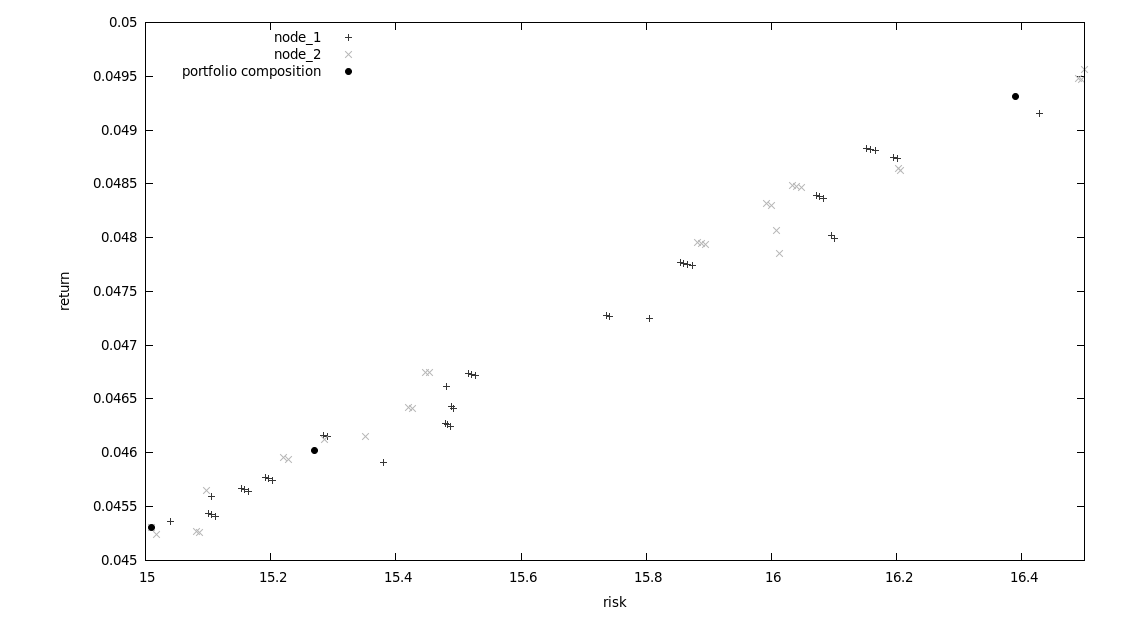
\includegraphics[scale=.3]{pareto_coemas.png}
  \end{center}
  \caption{Chart showing the relation between return and risk of the particular solution}
  \label{fig:pareto_coemas}
\end{figure}


\subsection{Conclusions}

First set of tests showed that all algorithms give reasonable results.
It is very hard to pinpoint one approach that is much better than others.
Co-evolutionary system (\ref{sec:co-evol-sys}) outperformed other algorithms in terms of return.
Such good results can be explained by the fact that trading strategy proposed by this algorithm is much riskier than using CoEMAS.
  
On the other hand, CoEMAS offers substantially lower return but is much more safer.
As figure~\ref{fig:agent_risk} shows, the risky moves are mixed with safe ones resulting in much more balanced strategy.

Trend following as well as genetic algorithm can not give us any information about the risk we are taking by investing according to results they provide.
On the other hand, we can specify rules (in the trend following approach) that should reflect our attitude to risk taking (\ref{sec:trend-following}).
With genetic algorithm (GA) we have no such option as our ability to customize GA is limited.
Obviously we could test different values of coefficients responsible for simulating evolution process but it turns out that the fitness function that does not take risk into
account is the most serious limitation.



\subsection{Second Set of Tests}

Third set of tests uses historical data from year 2008.
The same 3 companies stocks have been selected to construct our portfolio as in previous tests.
Year 2008 was extremely hard for investors due to crisis caused by credit crunch back in 2007.
During 2008, WIG 20 lost over 47\% in value.
Under such difficult circumstances it is tempting to run tests in order to asssess each algorithm ability to minimize losses.
The best solutions obtained as well as average ones are included.  

\subsection{Trend Following}

\subsubsection{Short-term trend results}

Algorithm is configured in the same manner as in \ref{short-term}.
Results are presented in figure~\ref{fig:trend_foll_short}.

\begin{figure}[htb]
  \subfigure[short-term trends]{
  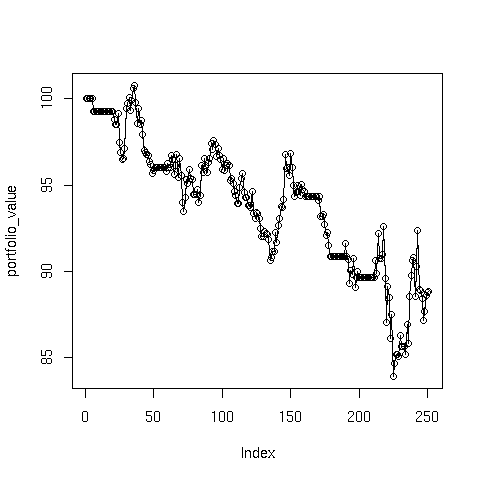
\includegraphics[scale=.33]{trend_following_short.png}
\label{fig:trend_foll_short}}
  \subfigure[intermediate-term trends]{
  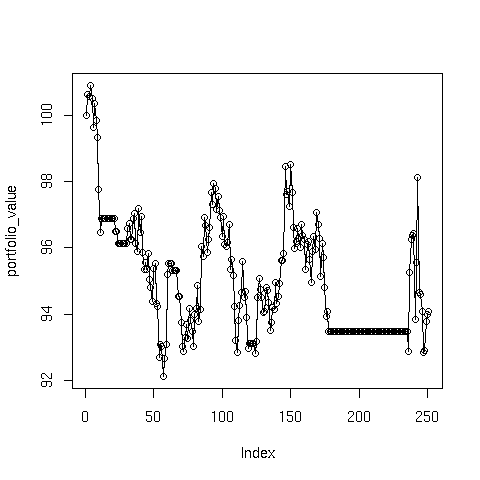
\includegraphics[scale=.33]{trend_following_inter.png}
  \label{fig:trend_foll_inter}
}
  \caption{Charts showing portfolio value in time for TF using short-term and intermediate-term trends}
\label{fig:TF_2}
\end{figure}

\subsubsection{Intermediate-term trend results}

Algorithm is configured in the same manner as in \ref{trend-foll-inter}.
Results are presented in figure~\ref{fig:trend_foll_inter}.


\subsubsection{Conclusions}

Intermediate-term trend seeking tends to give much better results than focusing on short-term trends.
We managed to minimize the losses thanks to the fact that we completely ceased trading during the worst time on the market.

\subsection{Genetic algorithm}

The best results that we were able to obtain are presented in figure ~\ref{fig:gen_ave_2008}.
Apart from that, the average values of 5 runs are shown in figure ~\ref{fig:gen_best_2008}.
As can be easily spotted the algorithm perform reasonably well on average (especially compared with CEA).

The following configuration was used:
\begin{itemize}
  \item $reproduction\_$ $coeff$ was set to 0.2;
  \item population size is 512;
  \item $mutation$ $\_$ $coeff$ was set to 0.1;
  \item $extinction$ $\_$ $coeff$ was set to 0.3.
\end{itemize}

\begin{figure}[htb]
  \subfigure[Chart showing average portfolio value in time]{
  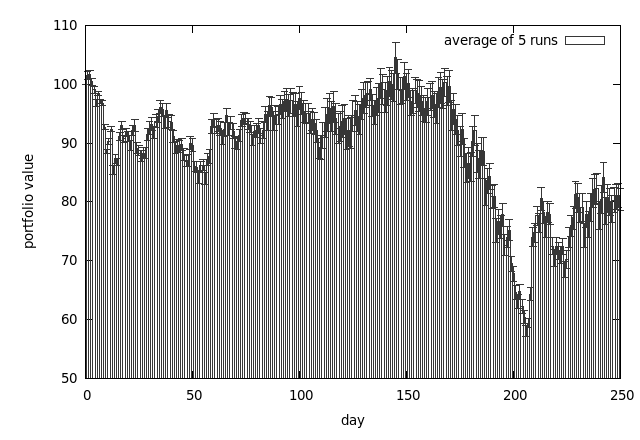
\includegraphics[scale=.3]{gen_ave_2008.png}
\label{fig:gen_ave_2008}}
  \subfigure[Chart showing best portfolio value in time]{
  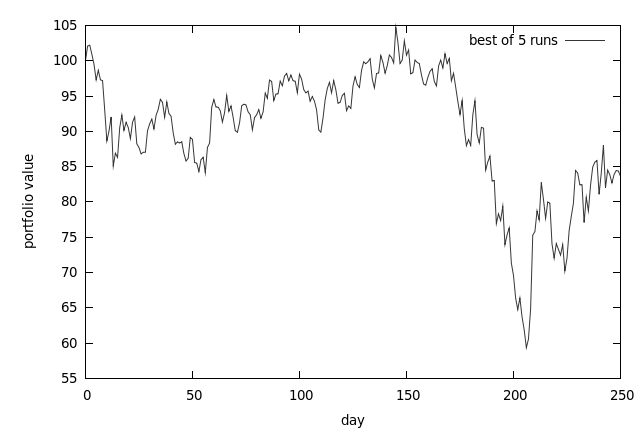
\includegraphics[scale=.3]{best_gen_2008.png}
  \label{fig:gen_best_2008}
}
  \caption{Charts showing portfolio value in time for GA}
\label{fig:GA_2}
\end{figure}

\subsection{Co-evolutionary algorithm}

Results presented in figure ~\ref{fig:co_evol_return} are catastrophic (and still they are the best results we obtained from a series of tests).
Average results are shown in figure ~\ref{fig:cea_2008_ave}

We have lost almost all our money - approximately 70\% of it.
Average risk associated with our portfolio is presented in figure ~\ref{fig:co-evol-risk}.
As we can observe the best obtained results are quite similar to average ones.

The following configuration was used:
\begin{itemize}
  \item $reproduction\_$ $coeff$ was set to 0.2;
  \item subpopulation size in each computing node was set to 64;
  \item number of computing nodes was set to 2;
  \item $mutation$ $\_$ $coeff$ was set to 0.1;
  \item $extinction$ $\_$ $coeff$ was set to 0.3.
\end{itemize}

\begin{figure}[htb]
  \subfigure[Chart showing best portfolio value in time]{
  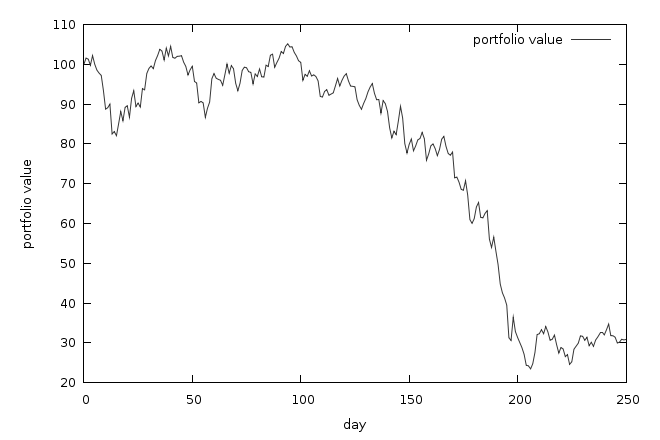
\includegraphics[scale=.3]{co-evol-return.png}
\label{fig:co_evol_return}}
  \subfigure[Chart showing average portfolio value in time]{
  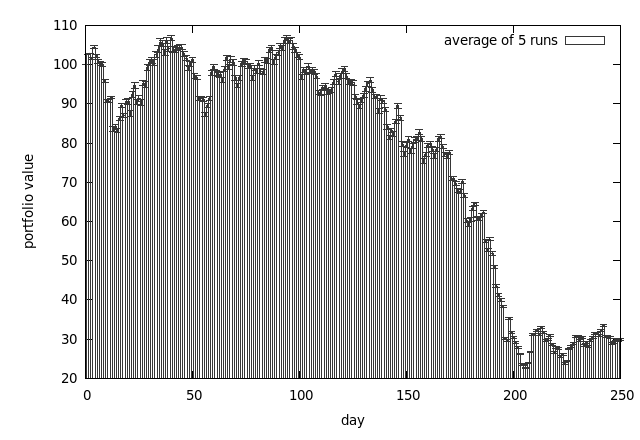
\includegraphics[scale=.3]{cea_2008_ave.png}
  \label{fig:cea_2008_ave}
}
  \caption{Charts showing portfolio value in time for CEA}
\label{fig:CEA_2}
\end{figure}


\subsection{CoEMAS}

Figure~\ref{fig:agent_2008_best_return} presents the best returns that we managed to obtain
  while  figure~\ref{fig:agent_2008_ave_return} presents the average risk associated with our investments.
Average return is shown in figure ~\ref{fig:agent_2008_ave_risk}.
Once again it turns out that average values are pretty similar to the best we managed to get. 
It turns out that CoEMAS performs much better in difficult times than CEA.

The following configuration was used:
\begin{itemize}
  \item $reproduction\_$ $coeff$ was set to 0.2;
  \item each species was represented initially by 64 agents (in each computing node);
  \item number of computing nodes was set to 2;
  \item $mutation$ $\_$ $coeff$ was set to 0.1;
  \item $extinction$ $\_$ $coeff$ was set to 0.3.
\end{itemize}

\begin{figure}[htb]
  \subfigure[Chart showing best portfolio value in time]{
  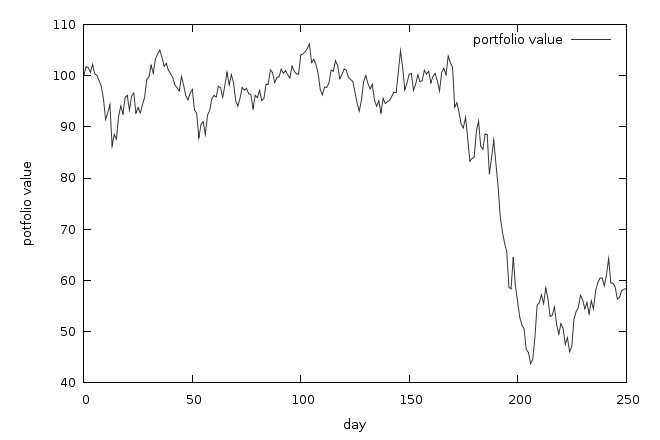
\includegraphics[scale=.3]{coemas-return.png}
\label{fig:agent_2008_best_return}}
  \subfigure[Chart showing average portfolio value in time]{
  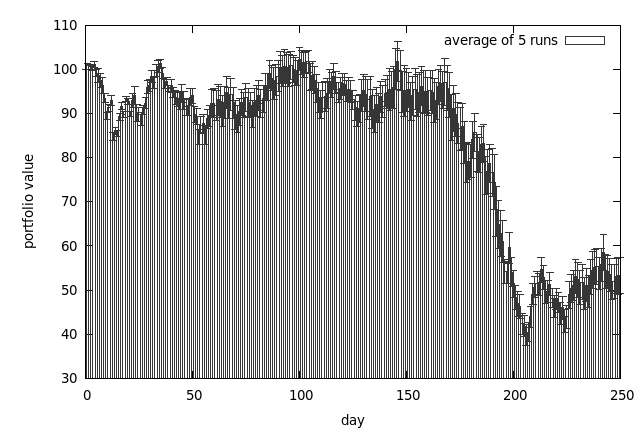
\includegraphics[scale=.3]{coemas_2008_ave.png}
  \label{fig:agent_2008_ave_return}
}
  \caption{Charts showing portfolio value in time for CoEMAS}
\label{fig:CoEMAS_2}
\end{figure}



\begin{figure}[htb]
  \subfigure[Chart showing average portfolio risk in time for CEA]{
  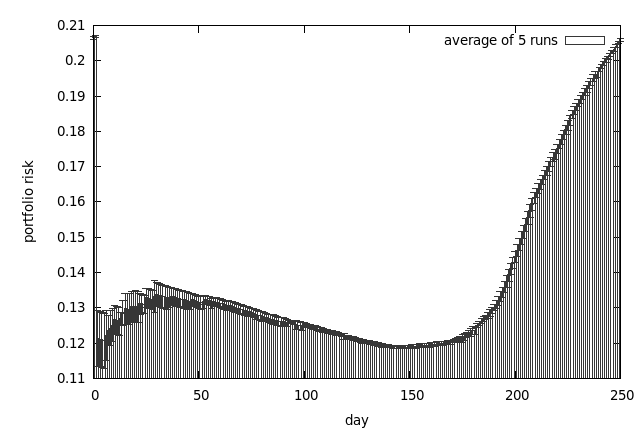
\includegraphics[scale=.3]{cea_2008_ave_risk.png}
\label{fig:co-evol-risk}}
  \subfigure[Chart showing average portfolio risk in time for CoEMAS]{
  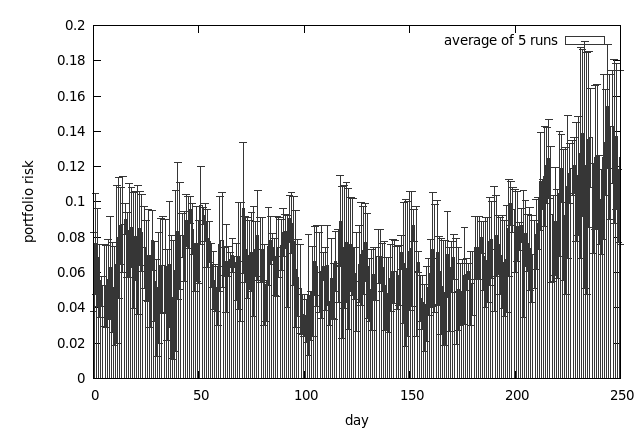
\includegraphics[scale=.3]{coemas_2008_ave_risk.png}
  \label{fig:agent_2008_ave_risk}
}
  \caption{Charts showing portfolio value in time for CoEMAS}
\label{fig:CoEMAS_CEA_2}
\end{figure}

\subsection{Conclusions}

Clearly, trend following approach managed to save almost our entire capital.
Losses that we had to experience due to this algorithm seems to be almost negligible comparing with other methods.

In spite of the fact that fitness function used in genetic algorithm completely ignores the risk associated with assets in portfolio,       it actually performed better then solution taking risk into consideration.

Co-evolutionary algorithm is particularly bad. 
Almost 70\% of initial money is lost. CoEMAS performs slightly better, but it is still worse than simple genetic algorithm approach.

Summing up, it turns out that algorithms performing exceptionally well in a bull market can potentially lead to catastrophic losses during
difficult times. 
Trend following algorithm has one major advantage among all discussed methods - it allows to withdraw all our money during periods of time
that are not investor friendly.

%%% -*- Coding: utf-8-unix; Mode: latex; TeX-master: "paper"; ispell-local-dictionary: "american" -*-

\section{Summary and Conclusions}
\label{sec:conclusions}

All implemented algorithms have been exhaustively tested using historical data reflecting completely different situations on the market.
Taking into consideration both good and bad times leads to conclusions that all approaches have advantages as well as disadvantages.
That raises a question what algorithm to use if we want to build our own portfolio.
Trend following is good for unstable times because it somehow guarantees that the losses would be minimalised according to our preferences.
However, during stock market rise it is outperformed by other algorithms.

\bibliographystyle{elsarticle-num}
\bibliography{ea-papers,ea-books}

\end{document}
